
\begin{figure}
\centering
\begin{subfigure}{.5\textwidth}
  \centering
  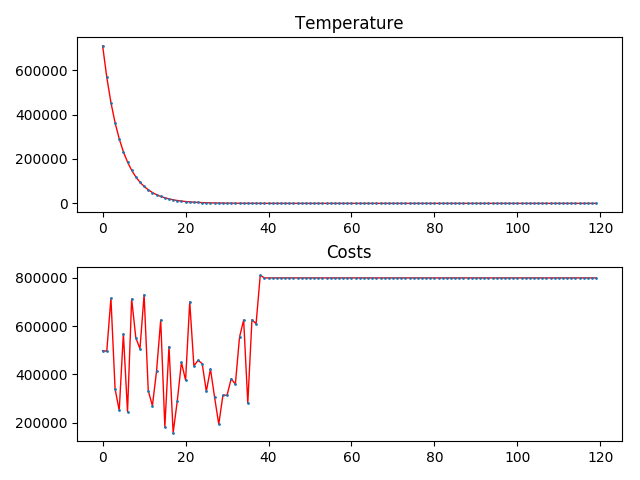
\includegraphics[width=1\linewidth]{results/cut12/1/plot}
  \label{fig:sub1}
\end{subfigure}%
\begin{subfigure}{.5\textwidth}
  \centering
  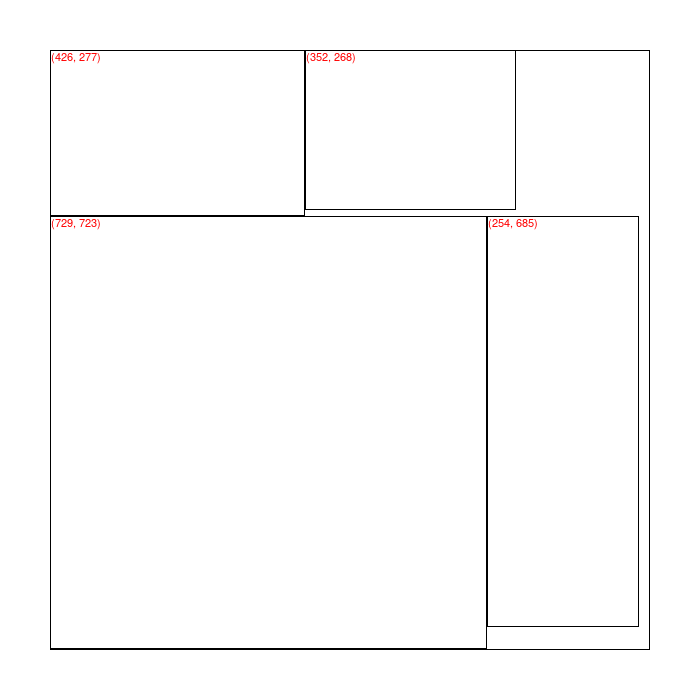
\includegraphics[width=1\linewidth]{results/cut12/1/cut}
  \label{fig:sub2}
\end{subfigure}
\caption{Instancia cut12.txt, 3.53\% de 1000x1000 (1000000)}
\label{fig:test}
\end{figure}


\begin{figure}
\centering
\begin{subfigure}{.5\textwidth}
  \centering
  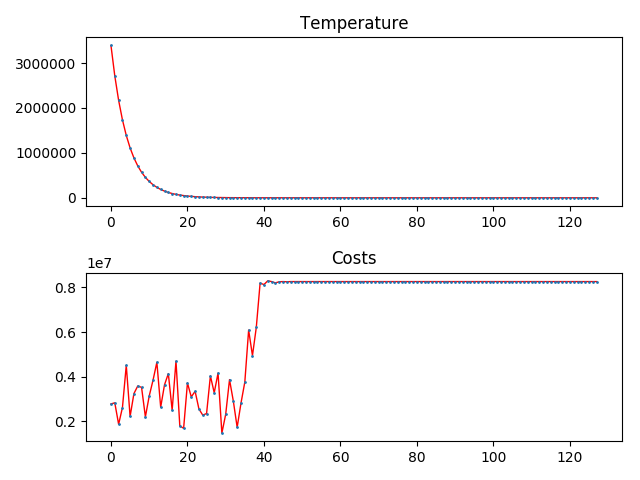
\includegraphics[width=1\linewidth]{results/cut13/3/plot}
  \label{fig:sub1}
\end{subfigure}%
\begin{subfigure}{.5\textwidth}
  \centering
  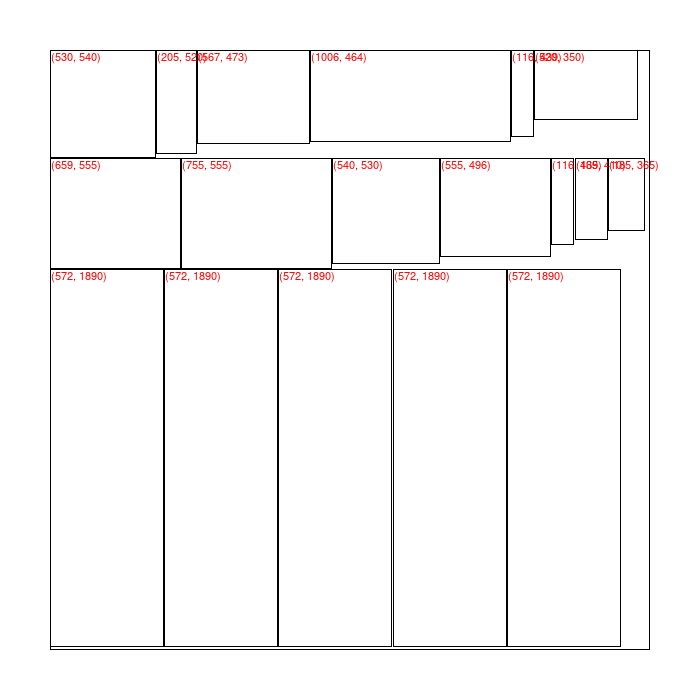
\includegraphics[width=1\linewidth]{results/cut13/3/cut}
  \label{fig:sub2}
\end{subfigure}
\caption{Instancia cut13.txt, 8.25\% de 3000x3000 (9000000)}
\label{fig:test}
\end{figure}


\begin{figure}
\centering
\begin{subfigure}{.5\textwidth}
  \centering
  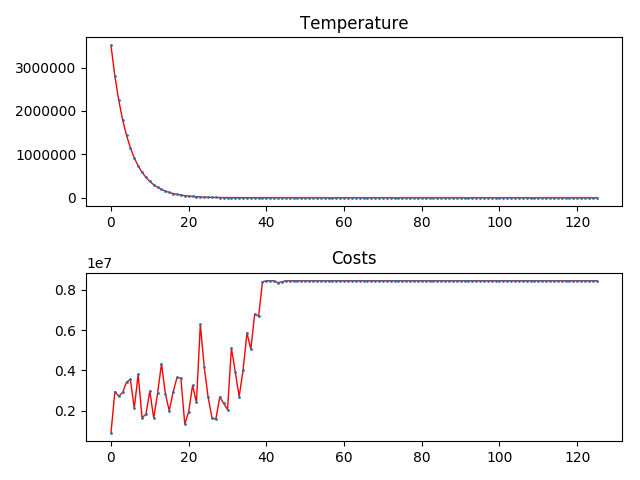
\includegraphics[width=1\linewidth]{results/cut14/2/plot}
  \label{fig:sub1}
\end{subfigure}%
\begin{subfigure}{.5\textwidth}
  \centering
  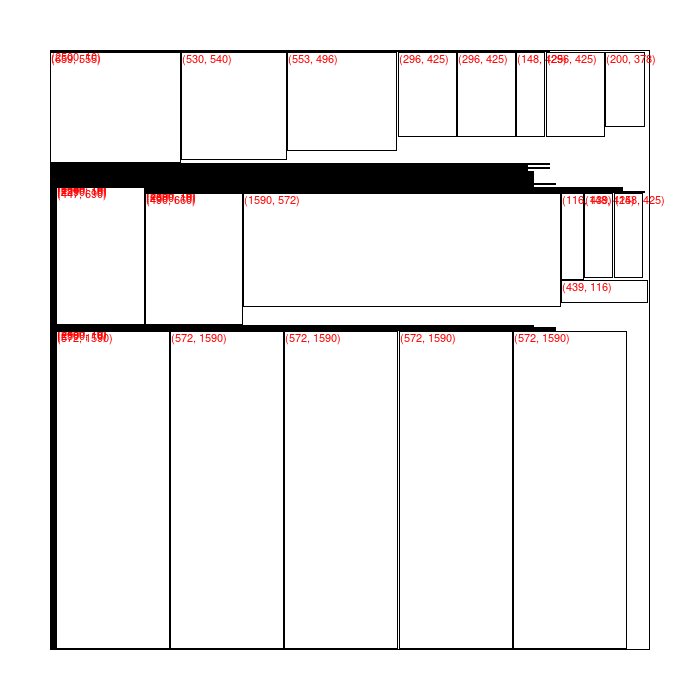
\includegraphics[width=1\linewidth]{results/cut14/2/cut}
  \label{fig:sub2}
\end{subfigure}
\caption{Instancia cut14.txt, 7.87\% de 3000x3000 (9000000)}
\label{fig:test}
\end{figure}


\begin{figure}
\centering
\begin{subfigure}{.5\textwidth}
  \centering
  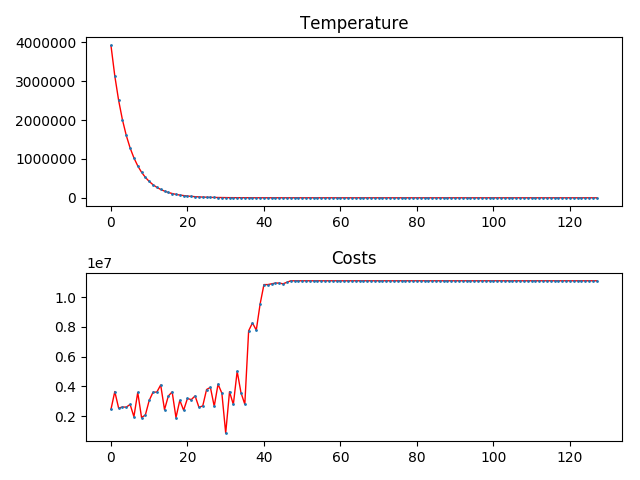
\includegraphics[width=1\linewidth]{results/cut17/2/plot}
  \label{fig:sub1}
\end{subfigure}%
\begin{subfigure}{.5\textwidth}
  \centering
  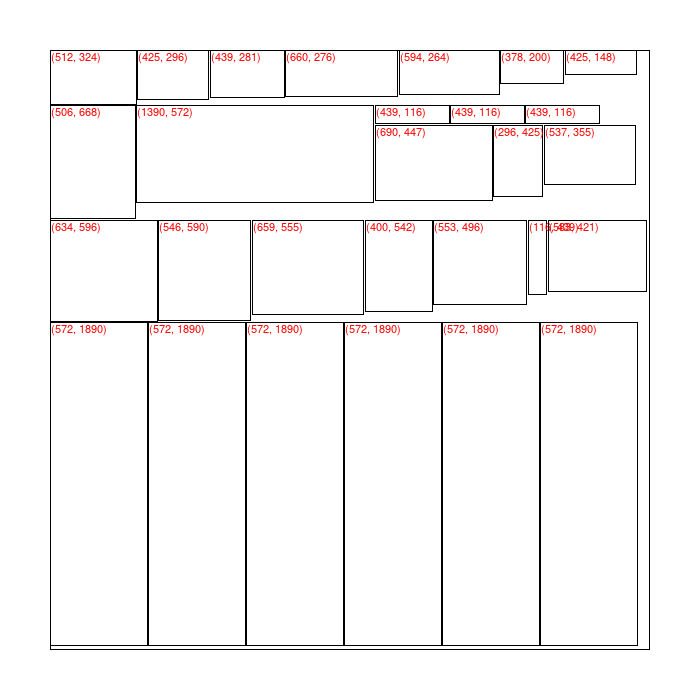
\includegraphics[width=1\linewidth]{results/cut17/2/cut}
  \label{fig:sub2}
\end{subfigure}
\caption{Instancia cut17.txt, 9.22\% de 3500x3500 (12250000)}
\label{fig:test}
\end{figure}


\begin{figure}
\centering
\begin{subfigure}{.5\textwidth}
  \centering
  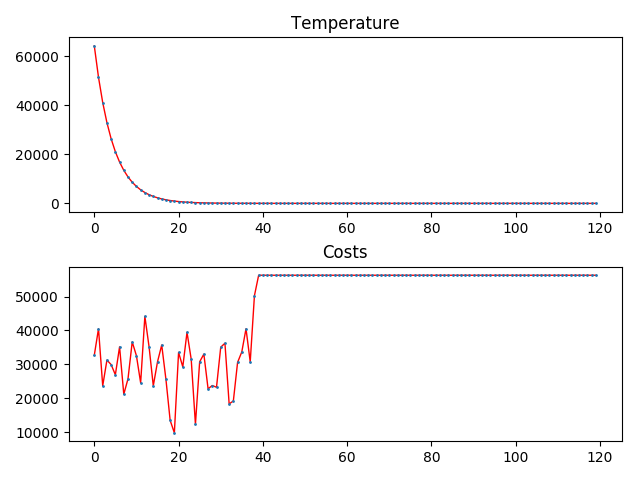
\includegraphics[width=1\linewidth]{results/cut1/2/plot}
  \label{fig:sub1}
\end{subfigure}%
\begin{subfigure}{.5\textwidth}
  \centering
  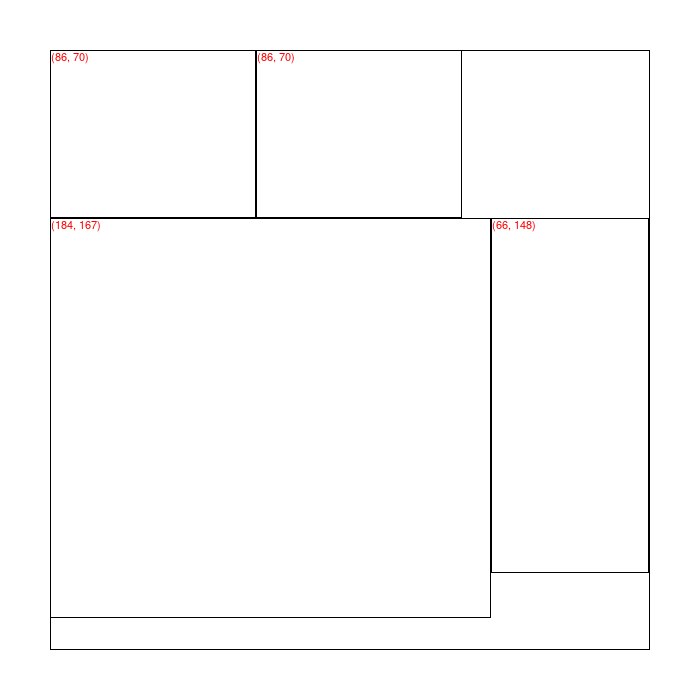
\includegraphics[width=1\linewidth]{results/cut1/2/cut}
  \label{fig:sub2}
\end{subfigure}
\caption{Instancia cut1.txt, 6.98\% de 250x250 (62500)}
\label{fig:test}
\end{figure}


\begin{figure}
\centering
\begin{subfigure}{.5\textwidth}
  \centering
  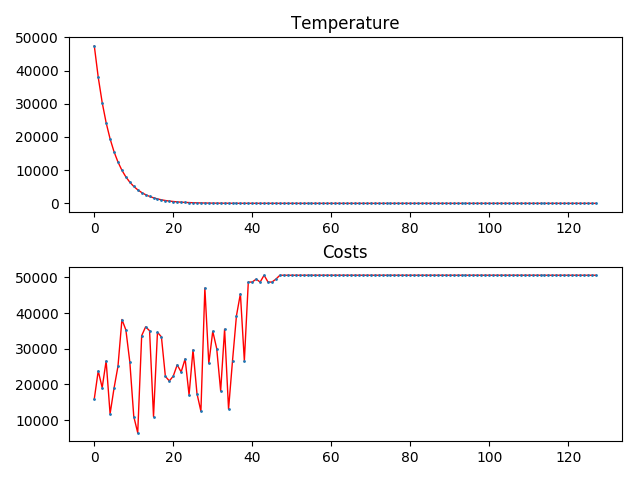
\includegraphics[width=1\linewidth]{results/cut2/3/plot}
  \label{fig:sub1}
\end{subfigure}%
\begin{subfigure}{.5\textwidth}
  \centering
  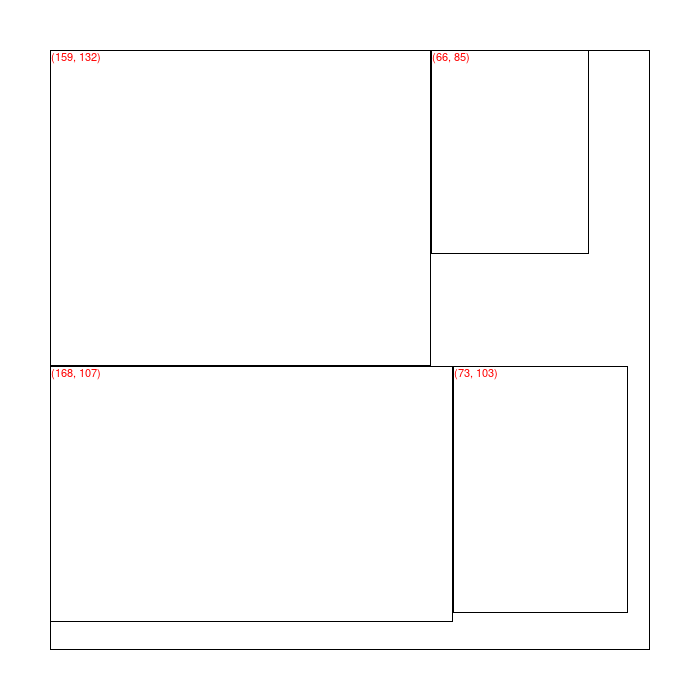
\includegraphics[width=1\linewidth]{results/cut2/3/cut}
  \label{fig:sub2}
\end{subfigure}
\caption{Instancia cut2.txt, 7.63\% de 250x250 (62500)}
\label{fig:test}
\end{figure}


\begin{figure}
\centering
\begin{subfigure}{.5\textwidth}
  \centering
  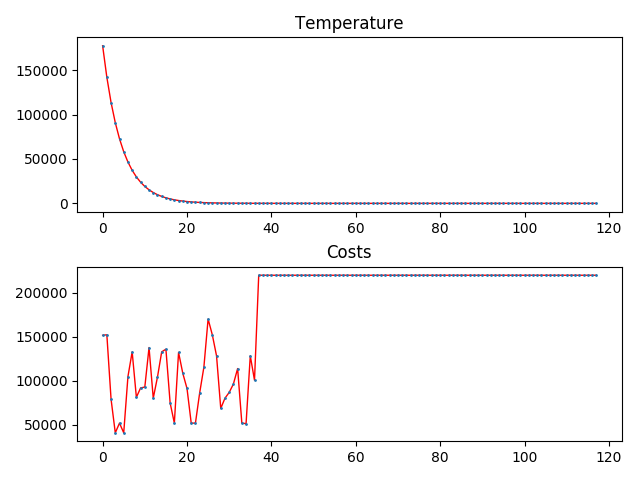
\includegraphics[width=1\linewidth]{results/cut5/3/plot}
  \label{fig:sub1}
\end{subfigure}%
\begin{subfigure}{.5\textwidth}
  \centering
  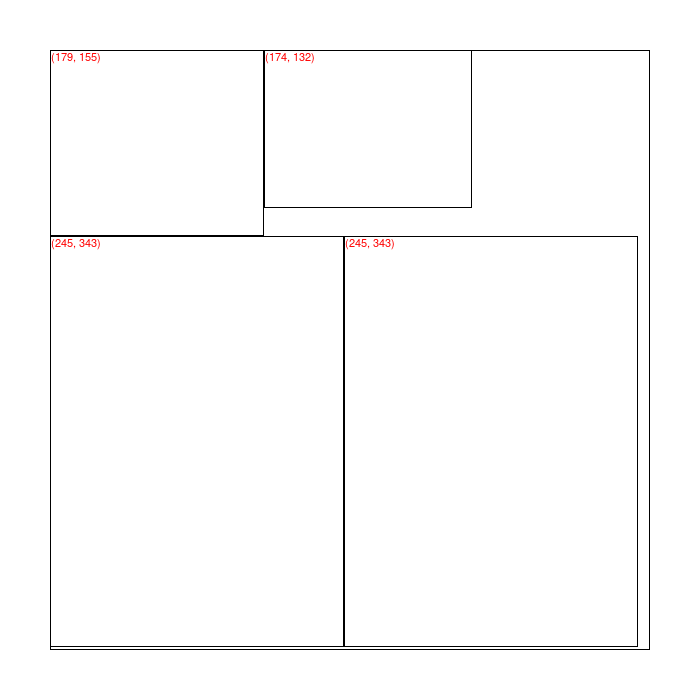
\includegraphics[width=1\linewidth]{results/cut5/3/cut}
  \label{fig:sub2}
\end{subfigure}
\caption{Instancia cut5.txt, 12.12\% de 500x500 (250000)}
\label{fig:test}
\end{figure}


\begin{figure}
\centering
\begin{subfigure}{.5\textwidth}
  \centering
  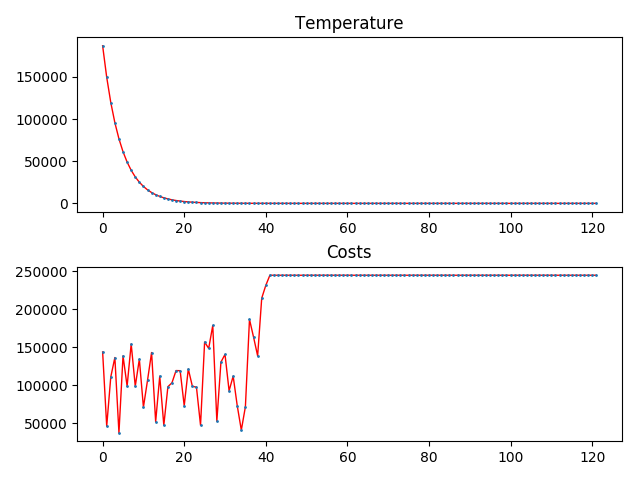
\includegraphics[width=1\linewidth]{results/cut7/1/plot}
  \label{fig:sub1}
\end{subfigure}%
\begin{subfigure}{.5\textwidth}
  \centering
  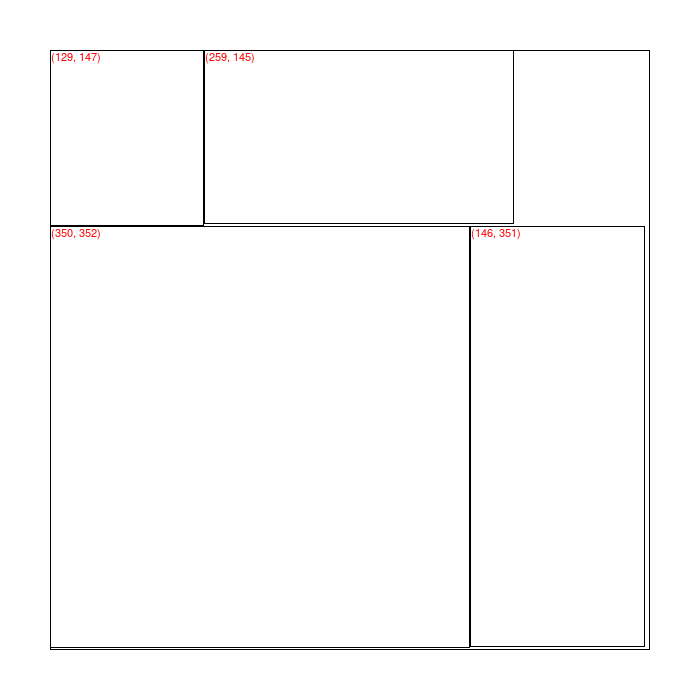
\includegraphics[width=1\linewidth]{results/cut7/1/cut}
  \label{fig:sub2}
\end{subfigure}
\caption{Instancia cut7.txt, 2.14\% de 500x500 (250000)}
\label{fig:test}
\end{figure}


\begin{figure}
\centering
\begin{subfigure}{.5\textwidth}
  \centering
  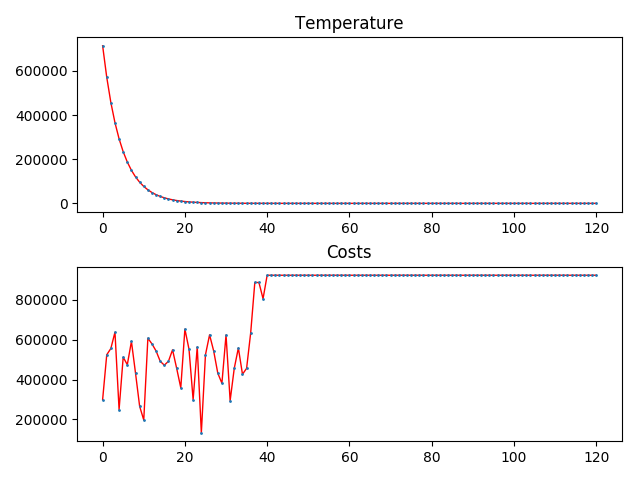
\includegraphics[width=1\linewidth]{results/cut9/1/plot}
  \label{fig:sub1}
\end{subfigure}%
\begin{subfigure}{.5\textwidth}
  \centering
  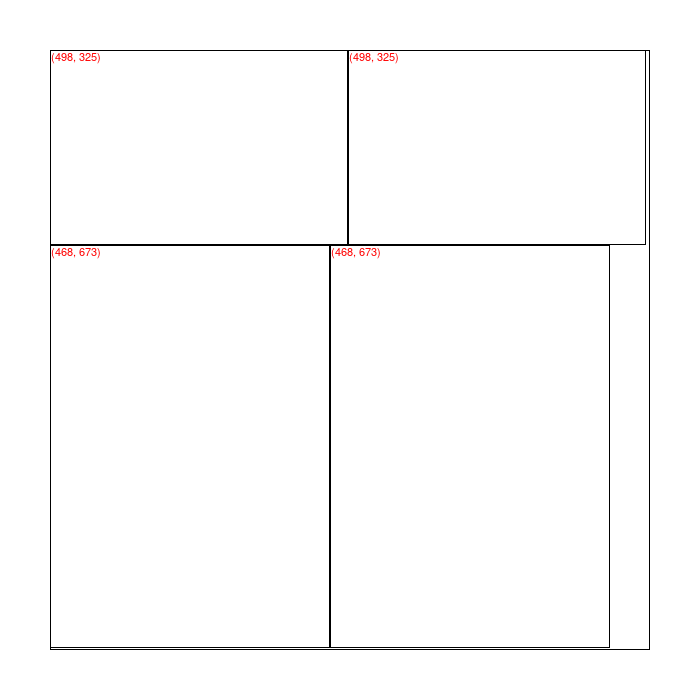
\includegraphics[width=1\linewidth]{results/cut9/1/cut}
  \label{fig:sub2}
\end{subfigure}
\caption{Instancia cut9.txt, 4.64\% de 1000x1000 (1000000)}
\label{fig:test}
\end{figure}

